\documentclass[a4paper, 12pt]{article}

% packages
\usepackage{amssymb}
\usepackage[fleqn]{mathtools}
\usepackage{tikz}
\usepackage{enumerate}
\usepackage{bussproofs}
\usepackage{xcolor}
\usepackage[margin=1.3cm]{geometry}
\usepackage{logicproof}
\usepackage{diagbox}
\usepackage{listings}
\usepackage{graphicx}
\usepackage{lstautogobble}
\usepackage{hyperref}
\usepackage{multirow}
\usepackage{tipa}
\usepackage{pgfplots}
\usepackage{adjustbox}

% tikz libraries
\usetikzlibrary{
    decorations.pathreplacing,
    arrows,
    shapes,
    shapes.gates.logic.US,
    circuits.logic.US,
    calc,
    automata,
    positioning,
    intersections
}

\pgfplotsset{compat=1.16}

\pgfmathdeclarefunction{gauss}{2}{%
  \pgfmathparse{1/(#2*sqrt(2*pi))*exp(-((x-#1)^2)/(2*#2^2))}%
}

\allowdisplaybreaks % allow environments to break
\setlength\parindent{0pt} % no indent

% shorthand for verbatim
% this clashes with logicproof, so maybe fix this at some point?
\catcode`~=\active
\def~#1~{\texttt{#1}}

% code listing
\lstdefinestyle{main}{
    numberstyle=\tiny,
    breaklines=true,
    showspaces=false,
    showstringspaces=false,
    tabsize=2,
    numbers=left,
    basicstyle=\ttfamily,
    columns=fixed,
    fontadjust=true,
    basewidth=0.5em,
    autogobble,
    xleftmargin=3.0ex,
    mathescape=true
}
\newcommand{\dollar}{\mbox{\textdollar}} %
\lstset{style=main}

% augmented matrix
\makeatletter
\renewcommand*\env@matrix[1][*\c@MaxMatrixCols c]{%
\hskip -\arraycolsep
\let\@ifnextchar\new@ifnextchar
\array{#1}}
\makeatother

% ceiling / floor
\DeclarePairedDelimiter{\ceil}{\lceil}{\rceil}
\DeclarePairedDelimiter{\floor}{\lfloor}{\rfloor}

% custom commands
\newcommand{\indefint}[2]{\int #1 \, \mathrm{d}#2}
\newcommand{\defint}[4]{\int_{#1}^{#2} #3 \, \mathrm{d}#4}
\newcommand{\pdif}[2]{\frac{\partial #1}{\partial #2}}
\newcommand{\dif}[2]{\frac{\mathrm{d}#1}{\mathrm{d}#2}}
\newcommand{\limit}[2]{\raisebox{0.5ex}{\scalebox{0.8}{$\displaystyle{\lim_{#1 \to #2}}$}}}
\newcommand{\limitsup}[2]{\raisebox{0.5ex}{\scalebox{0.8}{$\displaystyle{\limsup_{#1 \to #2}}$}}}
\newcommand{\summation}[2]{\sum\limits_{#1}^{#2}}
\newcommand{\product}[2]{\prod\limits_{#1}^{#2}}
\newcommand{\intbracket}[3]{\left[#3\right]_{#1}^{#2}}
\newcommand{\laplace}{\mathcal{L}}
\newcommand{\fourier}{\mathcal{F}}
\newcommand{\mat}[1]{\boldsymbol{#1}}
\renewcommand{\vec}[1]{\boldsymbol{#1}}
\newcommand{\rowt}[1]{\begin{bmatrix}
    #1
\end{bmatrix}^\top}
\DeclareMathOperator*{\argmax}{argmax}
\DeclareMathOperator*{\argmin}{argmin}

\newcommand{\lto}[0]{\leadsto\ }

\newcommand{\ulsmash}[1]{\underline{\smash{#1}}}

\newcommand{\powerset}[0]{\wp}
\renewcommand{\emptyset}[0]{\varnothing}

\makeatletter
\newsavebox{\@brx}
\newcommand{\llangle}[1][]{\savebox{\@brx}{\(\m@th{#1\langle}\)}%
  \mathopen{\copy\@brx\kern-0.5\wd\@brx\usebox{\@brx}}}
\newcommand{\rrangle}[1][]{\savebox{\@brx}{\(\m@th{#1\rangle}\)}%
  \mathclose{\copy\@brx\kern-0.5\wd\@brx\usebox{\@brx}}}
\makeatother
\newcommand{\lla}{\llangle}
\newcommand{\rra}{\rrangle}
\newcommand{\la}{\langle}
\newcommand{\ra}{\rangle}
\newcommand{\crnr}[1]{\text{\textopencorner} #1 \text{\textcorner}}
\newcommand{\bnfsep}[0]{\ |\ }
\newcommand{\concsep}[0]{\ ||\ }

\newcommand{\axiom}[1]{\AxiomC{#1}}
\newcommand{\unary}[1]{\UnaryInfC{#1}}
\newcommand{\binary}[1]{\BinaryInfC{#1}}
\newcommand{\trinary}[1]{\TrinaryInfC{#1}}
\newcommand{\quaternary}[1]{\QuaternaryInfC{#1}}
\newcommand{\quinary}[1]{\QuinaryInfC{#1}}
\newcommand{\dproof}[0]{\DisplayProof}
\newcommand{\llabel}[1]{\LeftLabel{\scriptsize #1}}
\newcommand{\rlabel}[1]{\RightLabel{\scriptsize #1}}

\newcommand{\ttbs}{\char`\\}
\newcommand{\lrbt}[0]{\ \bullet\ }

% colours
\newcommand{\violet}[1]{\textcolor{violet}{#1}}
\newcommand{\blue}[1]{\textcolor{blue}{#1}}
\newcommand{\red}[1]{\textcolor{red}{#1}}
\newcommand{\teal}[1]{\textcolor{teal}{#1}}

% reasoning proofs
\usepackage{ltablex}
\usepackage{environ}
\keepXColumns
\NewEnviron{reasoning}{
    \begin{tabularx}{\textwidth}{rlX}
        \BODY
    \end{tabularx}
}
\newcommand{\proofline}[3]{$(#1)$ & $#2$ & \hfill #3 \smallskip \\}
\newcommand{\proofarbitrary}[1]{& take arbitrary $#1$ \smallskip \\}
\newcommand{\prooftext}[1]{\multicolumn{3}{l}{#1} \smallskip \\}
\newcommand{\proofmath}[3]{$#1$ & = $#2$ & \hfill #3 \smallskip \\}
\newcommand{\prooftherefore}[1]{& $\therefore #1$ \smallskip \\}
\newcommand{\proofbc}[0]{\prooftext{\textbf{Base Case}}}
\newcommand{\proofis}[0]{\prooftext{\textbf{Inductive Step}}}

% ER diagrams
\newcommand{\nattribute}[4]{
    \node[draw, state, inner sep=0cm, minimum size=0.2cm, label=#3:{#4}] (#1) at (#2) {};
}
\newcommand{\mattribute}[4]{
    \node[draw, state, accepting, inner sep=0cm, minimum size=0.2cm, label=#3:{#4}] (#1) at (#2) {};
}
\newcommand{\dattribute}[4]{
    \node[draw, state, dashed, inner sep=0cm, minimum size=0.2cm, label=#3:{#4}] (#1) at (#2) {};
}
\newcommand{\entity}[3]{
    \node[] (#1-c) at (#2) {#3};
    \node[inner sep=0cm] (#1-l) at ($(#1-c) + (-1, 0)$) {};
    \node[inner sep=0cm] (#1-r) at ($(#1-c) + (1, 0)$) {};
    \node[inner sep=0cm] (#1-u) at ($(#1-c) + (0, 0.5)$) {};
    \node[inner sep=0cm] (#1-d) at ($(#1-c) + (0, -0.5)$) {};
    \draw
    ($(#1-c) + (-1, 0.5)$) -- ($(#1-c) + (1, 0.5)$) -- ($(#1-c) + (1, -0.5)$) -- ($(#1-c) + (-1, -0.5)$) -- cycle;
}
\newcommand{\relationship}[3]{
    \node[] (#1-c) at (#2) {#3};
    \node[inner sep=0cm] (#1-l) at ($(#1-c) + (-1, 0)$) {};
    \node[inner sep=0cm] (#1-r) at ($(#1-c) + (1, 0)$) {};
    \node[inner sep=0cm] (#1-u) at ($(#1-c) + (0, 1)$) {};
    \node[inner sep=0cm] (#1-d) at ($(#1-c) + (0, -1)$) {};
    \draw
    ($(#1-c) + (-1, 0)$) -- ($(#1-c) + (0, 1)$) -- ($(#1-c) + (1, 0)$) -- ($(#1-c) + (0, -1)$) -- cycle;
}

% AVL Trees
\newcommand{\avltri}[4]{
    \draw ($(#1)$) -- ($(#1) + #4*(0.5, -1)$) -- ($(#1) + #4*(-0.5, -1)$) -- cycle;
    \node at ($(#1) + #4*(0, -1) + (0, 0.5)$) {#3};
    \node at ($(#1) + #4*(0, -1) + (0, -0.5)$) {#2};
}

% RB Trees
\tikzset{rbtr/.style={inner sep=2pt, circle, draw=black, fill=red}}
\tikzset{rbtb/.style={inner sep=2pt, circle, draw=black, fill=black}}

% Samples
\tikzset{spos/.style={inner sep=2pt, circle, draw=black, fill=blue!20}}
\tikzset{sneg/.style={inner sep=2pt, circle, draw=black, fill=red!20}}

% Joins
\newcommand\ljoin{\stackrel{\mathclap{\normalfont\mbox{\tiny L}}}{\bowtie}}
\newcommand\rjoin{\stackrel{\mathclap{\normalfont\mbox{\tiny R}}}{\bowtie}}
\newcommand\ojoin{\stackrel{\mathclap{\normalfont\mbox{\tiny O}}}{\bowtie}}

\setcounter{MaxMatrixCols}{100}

% actual document
\begin{document}
    {\sc Computing $3^\text{rd}$ Year Notes} \hfill ~https://github.com/lin-e/imperial-revision~
    \rule{\textwidth}{0.1pt}
    \section*{CO333 - Robotics \hfill (60019)}
        \subsection*{Lecture 1 - Introduction to Robotics}
        \subsection*{Lecture 2 - Robot Motion}
            A definition of a robot is something that can \textbf{move} and \textbf{sense}, and uses some sort of information processing to link the two.
            Robots might want to move in the water, fly in the air, walk (legged) on land, or work in space.
            The course will focus on wheeled robots that work on generally flat surfaces.
            \subsubsection*{Coordinate Frames}
                \begin{center}
                    \begin{tikzpicture}
                        \node at (4, -0.5) {$x_W$};
                        \node at (-0.5, 4) {$y_W$};
                        \draw
                        (0, 0) edge[->] (4, 0)
                        (0, 0) edge[->] (0, 4)
                        (2, 0) edge[dashed] (2, 2)
                        (0, 2) edge[dashed] (2.75, 2);
                        \node[rbtb] at (2, 2) {};
                        \begin{scope}[shift={(1.8, 1.8)}]
                            \begin{scope}[rotate={45}]
                                \draw (-0.5, -0.5) -- (0.5, -0.5) -- (0.5, 0.5) -- (-0.5, 0.5) -- cycle;
                            \end{scope}
                        \end{scope}

                        \node at (3, 3.5) {$x_R$};
                        \node at (1, 3.5) {$y_R$};
                        \node at (3, 2.3) {$\theta_R$};
                        \draw
                        (2, 2) edge[->] (3, 3)
                        (2, 2) edge[->] (1, 3);
                        \draw (2, 2) ++(0:0.75) arc (0:45:0.75);
                    \end{tikzpicture}
                \end{center}
                We will be mostly focused on 2D coordinates, on the flat (close to planar) ground.
                The world frame $W$ is anchored in the world, and the robot frame $R$ is anchored to the robot (consider one point and orientation as the centre of the robot) - consider a set of axis carried by the robot.
                Often we are interested in the robot's location; the transformation between the world frame $W$ and the robot frame $R$.
            \subsubsection*{Degrees of Motion Freedom}
                This is to do with how many parameters we need to specify the aforementioned transformation, generally related to the number of dimensions the robot is moving in.
                The simplest is a single degree of freedom, where a train moves along the $x$-axis - this position can be specified in one parameter.
                A rigid body which moves on a ground plane, such as an AV or robot vacuum cleaner has 3 DoF; two translational ($x,y$) and one rotational (typically $\theta$).
                On the other hand, a rigid body which moves in 3D space has 6 degrees of freedom; three rotational and three rotational.
                \medskip

                A \textbf{holonomic robot} is able to move instantaneously in any direction in its space of DoF, otherwise it is \textbf{non-holonomic}.
                Most are non-holonomic, but some holonomic robots do exist; ground-based robots can be made with omnidirectional wheels.
                \medskip

                Standard wheel configurations (both non-holonomic; each has two motors but has three degrees of movement freedom, the number of control inputs are lower than the DoF) include;
                \begin{itemize}
                    \itemsep0em
                    \item \textbf{drive and steer} (car) - not implemented in this course
                        \smallskip

                        The combination of acceleration and braking determines how fast it moves forwards, and the orientation of wheel determines direction.
                        \begin{center}
                            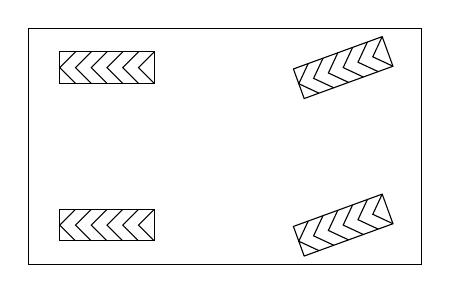
\begin{tikzpicture}
                                \draw (0, 0) -- (5, 0) -- (5, 3) -- (0, 3) -- cycle;
                                \begin{scope}[shift={(1, 2.5)}, scale={0.2}]
                                    \draw (-3, -1) -- (3, -1) -- (3, 1) -- (-3, 1) -- cycle;
                                    \foreach \i in {0,...,5} {
                                        \draw (\i - 2, 1) -- (\i - 3, 0) -- (\i - 2, -1);
                                    }
                                \end{scope}
                                \begin{scope}[shift={(1, 0.5)}, scale={0.2}]
                                    \draw (-3, -1) -- (3, -1) -- (3, 1) -- (-3, 1) -- cycle;
                                    \foreach \i in {0,...,5} {
                                        \draw (\i - 2, 1) -- (\i - 3, 0) -- (\i - 2, -1);
                                    }
                                \end{scope}
                                \begin{scope}[shift={(4, 2.5)}, rotate={20}, scale={0.2}]
                                    \draw (-3, -1) -- (3, -1) -- (3, 1) -- (-3, 1) -- cycle;
                                    \foreach \i in {0,...,5} {
                                        \draw (\i - 2, 1) -- (\i - 3, 0) -- (\i - 2, -1);
                                    }
                                \end{scope}
                                \begin{scope}[shift={(4, 0.5)}, rotate={20}, scale={0.2}]
                                    \draw (-3, -1) -- (3, -1) -- (3, 1) -- (-3, 1) -- cycle;
                                    \foreach \i in {0,...,5} {
                                        \draw (\i - 2, 1) -- (\i - 3, 0) -- (\i - 2, -1);
                                    }
                                \end{scope}
                            \end{tikzpicture}
                        \end{center}
                        Rear wheels need a differential, variable (Ackerman) linkage for steering wheels.
                    \item \textbf{differential drive} (robot vacuum)
                        \smallskip

                        Has two driving wheels, both pointing forwards, and maybe castors which keep it balanced.
                        Robot moves in different ways depending on the different speeds the wheels are turning at.
                        \begin{center}
                            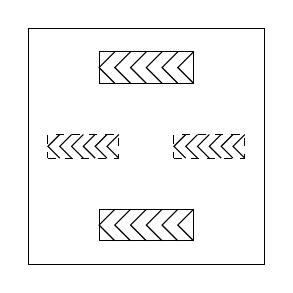
\begin{tikzpicture}
                                \draw (0, 0) -- (3, 0) -- (3, 3) -- (0, 3) -- cycle;
                                \begin{scope}[shift={(1.5, 2.5)}, scale={0.2}]
                                    \draw (-3, -1) -- (3, -1) -- (3, 1) -- (-3, 1) -- cycle;
                                    \foreach \i in {0,...,5} {
                                        \draw (\i - 2, 1) -- (\i - 3, 0) -- (\i - 2, -1);
                                    }
                                \end{scope}
                                \begin{scope}[shift={(1.5, 0.5)}, scale={0.2}]
                                    \draw (-3, -1) -- (3, -1) -- (3, 1) -- (-3, 1) -- cycle;
                                    \foreach \i in {0,...,5} {
                                        \draw (\i - 2, 1) -- (\i - 3, 0) -- (\i - 2, -1);
                                    }
                                \end{scope}
                                \begin{scope}[shift={(0.7, 1.5)}, scale={0.15}]
                                    \draw[dashed] (-3, -1) -- (3, -1) -- (3, 1) -- (-3, 1) -- cycle;
                                    \foreach \i in {0,...,5} {
                                        \draw (\i - 2, 1) -- (\i - 3, 0) -- (\i - 2, -1);
                                    }
                                \end{scope}
                                \begin{scope}[shift={(2.3, 1.5)}, scale={0.15}]
                                    \draw[dashed] (-3, -1) -- (3, -1) -- (3, 1) -- (-3, 1) -- cycle;
                                    \foreach \i in {0,...,5} {
                                        \draw (\i - 2, 1) -- (\i - 3, 0) -- (\i - 2, -1);
                                    }
                                \end{scope}
                            \end{tikzpicture}
                        \end{center}
                        The caster wheels (dashed) are passive, and simply support the robot.
                        The active wheels have one motor each.
                        If the active wheels are running at equal speeds, the robot moves in a straight line, and wheels running at equal and opposite speeds turn on the spot.
                        On the other hand, in general, other combinations lead to motion in circular arcs / curves.
                        \begin{center}
                            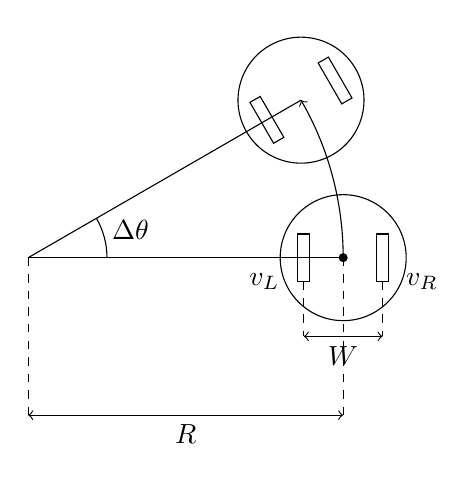
\begin{tikzpicture}
                                \begin{scope}
                                    \draw (4, 0) circle (0.8);
                                    \node[inner sep=1pt, circle, draw=black, fill=black] at (4, 0) {};
                                    \begin{scope}[shift={(3.5, 0)}, scale={0.15}]
                                        \draw (-0.5, -2) -- (-0.5, 2) -- (0.5, 2) -- (0.5, -2) -- cycle;
                                    \end{scope}
                                    \begin{scope}[shift={(4.5, 0)}, scale={0.15}]
                                        \draw (-0.5, -2) -- (-0.5, 2) -- (0.5, 2) -- (0.5, -2) -- cycle;
                                    \end{scope}
                                    \draw (0, 0) -- (4, 0);
                                \end{scope}
                                \begin{scope}[rotate={30}]
                                    \draw (4, 0) circle (0.8);
                                    \begin{scope}[shift={(3.5, 0)}, scale={0.15}]
                                        \draw (-0.5, -2) -- (-0.5, 2) -- (0.5, 2) -- (0.5, -2) -- cycle;
                                    \end{scope}
                                    \begin{scope}[shift={(4.5, 0)}, scale={0.15}]
                                        \draw (-0.5, -2) -- (-0.5, 2) -- (0.5, 2) -- (0.5, -2) -- cycle;
                                    \end{scope}
                                    \draw (0, 0) -- (4, 0);
                                \end{scope}
                                \draw (0, 0) ++(0:1) arc (0:30:1);
                                \draw[->] (0, 0) ++(0:4) arc (0:30:4);
                                \draw
                                (3.5, -1) edge[<->, below] node{$W$} (4.5, -1)
                                (0, -2) edge[<->, below] node{$R$} (4, -2);
                                \draw[dashed]
                                (0, 0) -- (0, -2)
                                (4, 0) -- (4, -2)
                                (3.5, -0.3) -- (3.5, -1)
                                (4.5, -0.3) -- (4.5, -1);
                                \node at (1.3, 0.35) {$\Delta \theta$};
                                \node at (3, -0.3) {$v_L$};
                                \node at (5, -0.3) {$v_R$};
                            \end{tikzpicture}
                        \end{center}
                        Consider the left wheel at speed $v_L$ and the right wheel at $v_R$ (linear velocities over th ground, hence $v_L = r_L\omega_L$, where $r_L$ is the radius of the wheel and $\omega_L$ is the angular velocity).
                        We also assume no slipping (the intersection is the centre of rotation).
                        \medskip

                        We want to determine $R$, which is the radius of the circle formed by the robot's centre moving.
                        Consider a small period of time $\Delta t$, and an angle of movement $\Delta \theta$;
                        $$\Delta \theta = \frac{v_L \Delta t}{R - \frac{W}{2}} = \frac{v_R \Delta t}{R + \frac{W}{2}} \Rightarrow v_L \left(R + \frac{W}{2}\right) = v_R \left(R - \frac{W}{2}\right) \Rightarrow \frac{W}{2}(v_L + v_R) = R(v_R - v_L)$$
                        By rearranging the above, and substituting back in, we have the following;
                        \begin{align*}
                            R & = \frac{W(v_R + v_L)}{2(v_R - v_L)} \\
                            \Delta \theta & = \frac{(v_R - v_L) \Delta t}{W}
                        \end{align*}
                \end{itemize}
            \subsubsection*{Actuation (DC Motors)}
                DC motors are controlled by a power signal, using \textbf{PWM (pulse width modulation)} and a fixed voltage.
                A gearing system is typically used to \textbf{gear down} the end effector to be slower with higher torque (compared to the DC motor's rapid rotation, but low torque).
                Many motors have a built in encoders (connected to the motor), which can be read to measure angular position by counting steps.
                This is required as a running motor's rotations depend on many conditions (including the load it's driving); for example a heavier robot moving on rough ground will move slower.
                To measure the rate the motor is moving at, we can feed the rotation back.
                We can then use feedback control (servo control) to adjust the motor to make it do what we want.
                In principle, we want to determine where the motor is, and where it actually is.
                At a high rate, we want to send pulses to reduce the error between the target location and actual location.
            \subsubsection*{PID (Proportional / Integral / Differential) Control}
                The PID expression sets the power as a function of error;
                $$P(t) = k_p e(t) + k_i \defint{0}{t}{e(\tau)}{\tau} + k_d \dif{e(t)}{t}$$
                In this, we have the following terms;
                \begin{itemize}
                    \itemsep0em
                    \item $e(t)$ \hfill demand minus position (error)
                        \smallskip

                        For example, at each time step this is the angle we want the motor to be at minus the actual angle of the motor measured.
                    \item $k_p$ \hfill main term (high values give rapid response)
                        \smallskip

                        Continuing with the example above, $k_p e(t)$ will be higher if $k_p$ is large.
                        If there's a large error, send a large signal, and vice versa for small errors.
                    \item $k_i$ \hfill integral term (increased to reduce steady state error)
                        \smallskip

                        Imagine the motor is close to where it should be; this allows for the `gap' to be closed.
                    \item $k_d$ \hfill differential term (reduced settling time / oscillation)
                \end{itemize}
            \subsubsection*{Wheel Rotation Speed to Velocity}
                Consider a wheel of radius $r_w$ rotating at $\omega$ (in radians per second).
                The speed of the wheel, in theory, would be $v = r_w \omega$.
                However, in practice, there are factors such as uneven ground and tyre softness, the radius may be hard to measure accurately.
                Another consideration would be possible slipping; in general it will be better to \textbf{calibrate} this for the surface by considering some constant of proportionality.
            \subsubsection*{State in 2D}
                If a robot is moving on a plane, we can define the robot with a state vector $\vec{x}$, with three parameters;
                $$\vec{x} = \begin{bmatrix}
                    x \\ y \\ \theta
                \end{bmatrix} \begin{matrix*}[l]
                    \text{$x$ component of robot centre point in world frame} \\
                    \text{$y$ component of robot centre point in world frame} \\
                    \text{rotation angle between coordinate frames (angle between $x_W$ and $x_R$ axes)}
                \end{matrix*}$$
                The two frames coincide when the robot is at the origin ($x = y = \theta = 0$).
                Note that $-\pi < \theta \leq \pi$.
                During a straight line period of motion of distance $D$, we have;
                $$\begin{bmatrix}
                    x^\prime \\
                    y^\prime \\
                    \theta^\prime
                \end{bmatrix} = \begin{bmatrix}
                    x + D \cos \theta \\
                    y + D \sin \theta \\
                    \theta
                \end{bmatrix}$$
                On the other hand, during a pure rotation of angle $\alpha$ we have (rotation to the left is positive by convention);
                $$\begin{bmatrix}
                    x^\prime \\
                    y^\prime \\
                    \theta^\prime
                \end{bmatrix} = \begin{bmatrix}
                    x \\
                    y \\
                    \theta + \alpha
                \end{bmatrix}$$
        \subsection*{Lecture 3 - Sensors (Behaviours)}
            \subsubsection*{Motivation}
                Recall the second practical; there was a gradual drift from the desired path.
                There are aspects of the world that the robot can never fully understand (such as the bumpiness of the floor) - even simulations cannot do exactly the same thing every time.
                After calibration, the robot should return to the desired location (on average), but some scatter will remain due to factors we cannot control.
                \medskip

                Systematic errors are removed, however we still have \textbf{zero mean errors} - these errors occur incrementally (where every movement or rotation adds a small amount of potential error).
                The zero mean errors can be modelled probabilistically, often with a Gaussian distribution.
            \subsubsection*{Uncertainty in Motion}
                A better model (compared to the previous lecture) adds uncertain perturbations / motion noise;
                $$\begin{bmatrix}
                    x^\prime \\
                    y^\prime \\
                    \theta^\prime
                \end{bmatrix} = \begin{bmatrix}
                    x + (D + e) \cos \theta \\
                    y + (D + e) \sin \theta \\
                    \theta + f
                \end{bmatrix}$$
                We will likely also notice that rotations are not exact either;
                $$\begin{bmatrix}
                    x^\prime \\
                    y^\prime \\
                    \theta^\prime
                \end{bmatrix} = \begin{bmatrix}
                    x \\
                    y \\
                    \theta + \alpha + g
                \end{bmatrix}$$
            \subsubsection*{Sensors}
                Proprioceptive are self-sensing (such as motor encoders / internal force sensors) and improve a robot's sense of its own internal state.
                In general, these measurements may depend on the previous states as (as well as the current state); for example wheel odometry gives a reading depending on a difference between the current and previous state, on the other hand, a gyro in an inertial measurement unit will report a reading depending on the current \textbf{rate} of rotation (not an instantaneous state).
                \medskip

                In this case, the value of the measurement $\vec{z}_p$ should be a function of the state of the state of the robot;
                $$\vec{z}_p = \vec{z}_p(\vec{x})$$

                On the other hand, exteroceptive are outward-looking.
                These allow the robot to generally be \textbf{aware} of its environment, letting it localise with respect to a map, recognise objects / locations, map out free space, avoid obstacles, and interact with objects.
                \medskip

                In this case, we need both the sate of the robot $\vec{x}$ and the state of the world $\vec{y}$ (relative to the robot);
                $$\vec{z}_o = \vec{z}_o(\vec{x}, \vec{y})$$
                The state of the world may be parameterised (such as a list of geometric coordinates describing landmarks).
                This state may be uncertain.
                \medskip

                Some sensors (such as touch, light, and sonar) will return a \textbf{single value} in a range.
                On the other hand, some sensors such as a camera or laser range-finder will return an \textbf{array} of values, with the former having an array of sensing elements (pixels of a camera's CCD chip), or the latter performing scanning.
                \medskip

                Some common sensors are as follows;
                \begin{itemize}
                    \itemsep0em
                    \item \textbf{touch sensor}
                        \smallskip

                        This is a binary on / off state; an open switch will have no current flow, and a closed switch will have current flow (hit).
                    \item \textbf{light sensor}
                        \smallskip

                        This detects intensity of passive light incident from a single forward direction (some range of angle sensitivity); this is a continuous value.
                        Multiple sensors can guide steering behaviours (such as driving towards a brighter light).
                        In \textit{Lego}, there is also a mode where the sensor can emit light, where reflections from close surfaces can be measured.
                    \item \textbf{sonar (ultrasonic) sensors}
                        \smallskip

                        Sonar measures distance by emitting ultrasonic pulses (tiny pulses of sound at a high frequency) - these beams typically have an angular width of $10^\circ - 20^\circ$.
                        The sensors measure the time for a pulse to bounce back (which the sensor uses to calculate the distance).
                        These are fairly accurate within a few centimetres in one direction (for simple shapes) - but can be noisy in the presence of complicated shapes.
                        The maximum range is a few metres.
                    \item \textbf{laser range-finder}
                        \smallskip

                        The principle of this is similar to sonar, however it uses infrared laser beams instead of sound.
                        This is also reflected, detected, and timed to calculate a distance.
                        These are very accurate (sub-millimetre), and work on most surfaces.
                        They can normally scan in a 2D plane (rotating on one axis), but can also scan in 3D.
                        Previously, these were bulky and expensive, however nowadays they are present in modern smartphones.
                \end{itemize}
            \subsubsection*{Vision}
                This is the generalisation of a light sensor.
                A camera can be thought of as a large array of light sensors (or a light sensor is a single pixel of) which returns a large, rectangular array of measurements.
                A single camera measures light intensity (rather than direct information about geometry).
            \subsubsection*{Bump Detection (Touch Sensor)}
                We can either perform this with a touch sensor, or by thresholding sonar (such as if the distance falls below some range).
                \medskip

                Multiple touch sensors mounted inside a floating skirt can allow for detection of where an obstacle was hit.
                For example, if a robot was hit at the front, it may attempt to drive around it by going backwards, moving around, and continuing.
                Another simple strategy is to rotate through a random angle and go forward until the next collision (random bounce).
            \subsubsection*{Servoing}
                Servoing is a control technique where control parameters (e.g. the desired speed of a motor) are coupled directly to a sensor reading and updated regularly in a \textbf{negative feedback loop} - this is also known as \textbf{closed loop control}.
                This requires high frequency updates of both the sensor and the update, otherwise the motion can oscillate.
                \medskip

                Propeortional control sets the demand proportional to negative error - for example in velocity (where we look at the difference between the desired sensor value and actual sensor value);
                $$v = -k_p (z_\text{desired} - z_\text{actual})$$
                This proportional case is a specific case of PID control.
                \medskip

                A simple steering law to guide the robot to collide with the target would be as follows (for example - if the obstacle is straight ahead ($\alpha = 0$), then don't steer);
                $$s = k_p \alpha$$
                On the other hand, to guide the robot to avoid the obstacle at a safe distance ($R$) would subtract an offset ($D$ is the distance from the robot to the object, and $\alpha$ is the angle between the robot's rotation and the direction to the object);
                $$s = k_p(\alpha - \sin^{-1}\frac{R}{D})$$
            \subsubsection*{Wall Following}
                Consider the following scenario, where a differential drive robot desires to travel along a wall, at some distance $d$.
                This uses a \textbf{sideways-looking sonar} to measure some distance $z$.
                In the following diagram, the wall can be curved; I just don't know how to do that in TikZ.
                \begin{center}
                    \begin{tikzpicture}
                        \draw (-3, 3) -- (10, 3);
                        \begin{scope}[scale={0.5}]
                            \draw (0, 0) -- (3, 0) -- (3, 3) -- (0, 3) -- cycle;
                            \begin{scope}[shift={(1.5, 2.5)}, scale={-0.2}]
                                \draw (-3, -1) -- (3, -1) -- (3, 1) -- (-3, 1) -- cycle;
                                \foreach \i in {0,...,5} {
                                    \draw (\i - 2, 1) -- (\i - 3, 0) -- (\i - 2, -1);
                                }
                            \end{scope}
                            \begin{scope}[shift={(1.5, 0.5)}, scale={-0.2}]
                                \draw (-3, -1) -- (3, -1) -- (3, 1) -- (-3, 1) -- cycle;
                                \foreach \i in {0,...,5} {
                                    \draw (\i - 2, 1) -- (\i - 3, 0) -- (\i - 2, -1);
                                }
                            \end{scope}
                            \begin{scope}[shift={(0.7, 1.5)}, scale={-0.15}]
                                \draw[dashed] (-3, -1) -- (3, -1) -- (3, 1) -- (-3, 1) -- cycle;
                                \foreach \i in {0,...,5} {
                                    \draw (\i - 2, 1) -- (\i - 3, 0) -- (\i - 2, -1);
                                }
                            \end{scope}
                            \begin{scope}[shift={(2.3, 1.5)}, scale={-0.15}]
                                \draw[dashed] (-3, -1) -- (3, -1) -- (3, 1) -- (-3, 1) -- cycle;
                                \foreach \i in {0,...,5} {
                                    \draw (\i - 2, 1) -- (\i - 3, 0) -- (\i - 2, -1);
                                }
                            \end{scope}
                        \end{scope}
                        \draw (0.75, 0.75) edge[->, right] node{$v$} (0.75, 3);
                        \draw (-0.1, 1.5) edge[<->, left] node{$d$} (-0.1, 3);
                    \end{tikzpicture}
                \end{center}
                Note that we are moving left to right (along the diagram), and we want to steer towards the wall (since we'd ideally have $d = v$).
                To do this, the left wheel must turn slower than the right wheel.
                Note that we can also achieve symmetric behaviour with a constant offset $v_C$ (standard speed for a straight line).
                We can then set the left and right wheel velocities as follows;
                \begin{align*}
                    v_R - v_L & = k_p(z - d) \\
                    v_R & = v_C + \frac{1}{2}k_p(z - d) \\
                    v_L & = v_C - \frac{1}{2}k_p(z - d)
                \end{align*}
            \subsubsection*{Combining}
                More complex robots may have multiple servos, and we can combine sensing-action loops.
                We can instead consider each local servo-like sensing-action loop as a \textbf{behaviour}.
                These behaviours can then be combined in an \textbf{arbiter}, which feeds the instructions into a motor controller.
                \medskip

                To go further, we need to go beyond a coupling between sensors and actions, and instead build a model of the world.
                Here we plan a sequence of actions to achieve a goal, and then execute the plan.
                However, if the world changes during the execution, we need to re-plan the actions.
        \subsection*{Lecture 4 - Probabilistic Robotics}
        \subsection*{Lecture 5 - Monte Carlo Localisation}
        \subsection*{Lecture 6 - Advanced Sonar Sensing}
        \subsection*{Lecture 7 - SLAM}
\end{document}